\clearpage
\sffamily
{\bfseries\color[rgb]{0.4,0.4,0.4}
Part A: Push Recovery \added{AdultSize only}}
\phantomsection
\addcontentsline{toc}{subsection}{Part A: Push Recovery (AdultSize only)}


\bigskip

The goal of the push recovery challenge is to withstand a strong push while walking. 

Cushioned plastic bottles partially filled with sand (or similar) will be suspended on a rope of fixed length, and swung into the robot as a pendulum to apply the push. Bottles of mass 1$\,$kg, 2$\,$kg, 3$\,$kg and 5$\,$kg will be available, where the default mass to use in each size class will be 1$\,$kg in KidSize, 2$\,$kg in TeenSize and 3$\,$kg in AdultSize. If a robot completes a fully successful trial with the default mass for its size class, then a larger bottle may be used in further trials.

\medskip
The length of the rope $L$ (between 1.5 and 2 meters, measured from the point of 
attachment to the centre of mass of the bottle) will remain fixed for all trials 
of a particular size class.
The rope is attached to a frame of adjustable height,
which is used to adjust the centre of mass of the bottle at the moment of impact
to be as close as possible to the height of the centre of mass of the robot.
Where this is not possible, the centre of mass of the bottle should strike a solid part
of the centre of the hips of the robot.
For this and other purposes, the centre of mass of the bottle should be clearly marked.

\medskip
Each trial consists of three pushes---a push from the front, a push from the back, and a push from either the front or the back, in any order. To apply a push, the bottle is released from a particular position, and allowed to swing into the robot in such a way that the impact occurs when the rope is vertical. The amount of retraction of the bottle is measured by the ground projected distance $D$ from the centre of mass of the bottle, to the attachment point of the rope. Before each trial (set of three pushes), the team must declare what value of $D$ should be used (limited to $0.75L$ for practical implementation concerns). A push is successfully absorbed if after receiving the push the robot 
returns to a stable walking cycle, as perceived by the referee. The robot must be walking in place (with a normal step frequency) both before the push, and after it has stabilised itself again.

\medskip
For a complete trial to be fully successful, the robot needs to successfully absorb all three pushes. For a trial to be partially successful, the robot needs to successfully absorb two of the three pushes. The robots are ranked by the following metric (higher is better):
\begin{align*}
M = \frac{\sqrt{H}}{h_c} \cdot \frac{m_B}{m_R} \cdot \frac{h_i}{h_c}
\end{align*}
where we have the following:
\begin{center}
\begin{tabular}{l@{\hspace{1.2em}}l@{\hspace{4em}}l@{\hspace{1.2em}}l}
$M$ & Ranking metric & $H$ & Vertical height fallen by the bottle $=L - \sqrt{L^{2} - D^{2}}$  \\
$m_B$ & Mass of the bottle & $h_i$ & Height of the centre of mass of the bottle at impact \\
$m_R$ & Mass of the robot & $h_c$ & Height of the centre of mass of the robot \\
\end{tabular}
\end{center}  

\begin{figure}[h]
\begin{center}
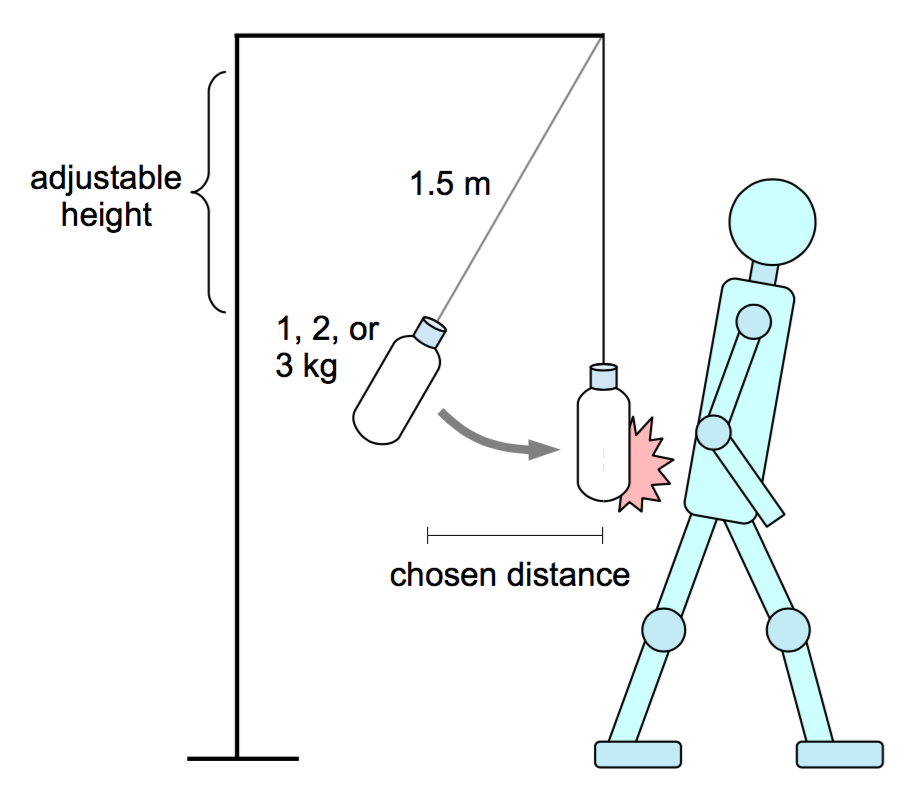
\includegraphics[height=6.5cm]{img/push_recovery.png}
\caption{Setup for the push recovery challenge. }
\end{center}
\end{figure}
